% Author: Izaak Neutelings (October 2020)
\documentclass[border=3pt,tikz]{standalone}
\usepackage{physics}
\usepackage{tikz}
\usepackage[outline]{contour} % glow around text
\usetikzlibrary{calc}
\usetikzlibrary{angles,quotes} % for pic
\usetikzlibrary{patterns,snakes}
\tikzset{>=latex} % for LaTeX arrow head
\contourlength{1.1pt}

\colorlet{xcol}{blue!98!black}
\colorlet{xcoldark}{blue!50!black}
\colorlet{vcol}{green!70!black}
\colorlet{myred}{red!80!black}
\colorlet{mypurple}{blue!60!red!80}
\colorlet{acol}{red!50!blue!80!black!80}
\tikzstyle{rvec}=[->,xcol,very thick,line cap=round]
\tikzstyle{force}=[->,myred,very thick,line cap=round]
\tikzstyle{mass}=[line width=0.6,red!30!black,fill=red!40!black!10,rounded corners=1,
                  top color=red!40!black!20,bottom color=red!40!black!10,shading angle=20]

\tikzset{
  pics/Tin/.style={
    code={
      \def\R{0.12}
      \draw[pic actions,line width=0.6,#1,fill=white] % ,thick
        (0,0) circle (\R) (-135:.75*\R) -- (45:.75*\R) (-45:.75*\R) -- (135:.75*\R);
  }},
  pics/Tout/.style={
    code={
      \def\R{0.12}
      \draw[pic actions,line width=0.6,#1,fill=white] (0,0) circle (\R);
      \fill[pic actions,#1] (0,0) circle (0.3*\R);
  }},
  pics/Tin/.default=mypurple,
  pics/Tout/.default=mypurple,
}

\newcommand\rightAngle[4]{
  \pgfmathanglebetweenpoints{\pgfpointanchor{#2}{center}}{\pgfpointanchor{#3}{center}}
  \coordinate (tmpRA) at ($(#2)+(\pgfmathresult+45:#4)$);
  \draw[white,line width=0.7] ($(#2)!(tmpRA)!(#1)$) -- (tmpRA) -- ($(#2)!(tmpRA)!(#3)$);
  \draw[xcoldark] ($(#2)!(tmpRA)!(#1)$) -- (tmpRA) -- ($(#2)!(tmpRA)!(#3)$);
}

% BICYCLE WHEEL
\def\r{0.16}  % axis radius
\def\Ri{1.18} % wheel rims inside
\def\Rr{1.30} % wheel rims outside
\def\Rt{1.45} % wheel tyre
\def\wheel{
  \def\Ns{11}   % number of spokes
  \def\Nn{34}   % number of tyre stud
  \coordinate (O) at (0,0);
  \foreach \i [evaluate={\ang=\i*360/(\Ns+1);}] in {0,...,\Ns}{
    \draw[line width=0.5,black!70,line cap=round] (\ang-90:\r) --++ (\ang:\Rr);
  }
  \draw[very thin,fill=black!30] (O) circle (1.2*\r);
  \draw[very thin,black!70] (O) circle (0.6*\r) circle (0.3*\r);
  \foreach \i [evaluate={\ang=\i*360/(\Ns+1);}] in {0,...,\Ns}{
    \fill (\ang+90:\r) circle (0.015);
    \draw[line width=0.5,black!70,line cap=round] (\ang+90:\r) --++ (\ang:\Rr);
  }
  \draw[fill=black!30,even odd rule] (O) circle (\Ri) circle (\Rr);
  
  \draw[fill=black!84,even odd rule] (O) circle (\Rr) (\Rt,0)
    \foreach \i [evaluate={\anga=\i*360/(\Nn+1);\angb=(\i+0.5)*360/(\Nn+1);
                           \angc=(\i+1)*360/(\Nn+1);}] in {0,...,\Nn}{
      -- (\anga:1.008*\Rt) arc(\anga:\angb:1.008*\Rt)
      -- (\angb:1.000*\Rt) arc(\angb:\angc:1.000*\Rt)
    } -- cycle;
  \draw[very thin] (O) circle (0.97*\Rt) circle (0.945*\Rt);
}

\begin{document}


% TORQUE perpendicular
\def\R{1.6} % wheel rims inside
\begin{tikzpicture}
  \def\ang{90} % angle
  \def\F{1.2}  % force size
  \coordinate (O) at (0,0);
  \coordinate (R) at (\ang:\R);
  \clip (-1.2*\Rr,-1.17*\Rr) rectangle (1.17*\Rr,1.54*\Rr);
  \wheel
  \draw[force] (R) --++ (\ang+90:\F) node[left=-2] {$\vb{F}$};
  \pic[scale=1] at (R) {Tout};
  \node[mypurple,above=2] at (R) {$\vb*\tau$};
  \draw[rvec] (O) -- (\ang:0.95*\R) node[midway,above=3,right=-1] {\contour{white}{$\vb{r}$}};
\end{tikzpicture}


% TORQUE parallel
\begin{tikzpicture}
  \def\ang{90} % angle
  \def\F{0.9}  % force size
  \coordinate (O) at (0,0);
  \coordinate (R) at (\ang:\R);
  \clip (-1.2*\Rr,-1.17*\Rr) rectangle (1.17*\Rr,1.54*\Rr);
  \wheel
  \node[mypurple,above=0] at (R) {$\vb*\tau = 0$};
  \draw[force] (R)++(\ang+110:0.16) --++ (\ang-180:\F) node[below left=-3] {\contour{white}{$\vb{F}$}};
  \draw[rvec] (O) -- (\ang:0.95*\R) node[midway,above=2,right=-1] {\contour{white}{$\vb{r}$}};
\end{tikzpicture}


% TORQUE angle
\begin{tikzpicture}
  \def\ang{43} % angle position
  \def\angF{8} % angle force
  \def\F{1.1}  % force size
  \coordinate (O) at (0,0);
  \coordinate (R) at (\ang:\R);
  \coordinate (RT) at (90+\angF:{\R*sin(\ang-\angF)});
  \coordinate (R') at (2*\ang-180-\angF:\R);
  \coordinate (F) at ($(R)+(\angF:\F)$);
  \coordinate (FT) at ($(R)+(\ang-90:{\F*sin(\ang-\angF)})$);
  \clip (-1.2*\Rr,-1.17*\Rr) rectangle (2.04*\Rr,1.54*\Rr);
  \wheel
  \rightAngle{R}{RT}{O}{0.40}
  \rightAngle{R}{FT}{F}{0.35}
  \draw[line width=0.8,dashed,white] (R) -- (RT) (R) --++ (\ang:0.4*\R) coordinate (RE); %line cap=round
  \draw[line width=0.5,dashed,xcol] (R) -- (RT) --++ (180+\angF:0.3) (R) --++ (\ang:0.5*\R);
  \draw[force] (R) -- (F) node[right=-2] {$\vb{F}$};
  \draw[force,myred!80!black!60]
    (R) -- (FT) coordinate (FT) node[below right=-3] {$\vb{F}_\mathrm{t}$};
  \pic[scale=1] at (R) {Tin};
  \draw[dashed,red!20!black] (F) -- (FT);
  \node[mypurple,above=2] at (R) {$\vb*\tau$};
  \draw[rvec,xcol!90!black!50] (O) -- (RT) node[midway,above=3,left=-2] {\contour{white}{$\vb{r}_\mathrm{t}$}};
  \draw[rvec] (O) -- (\ang:0.95*\R) node[midway,below=2,right=1] {\contour{white}{$\vb{r}$}};
  \draw pic["$\theta$",xcoldark,draw=xcoldark,angle radius=14,angle eccentricity=1.4] {angle=F--R--RE};
  \draw pic[thick,draw=white,angle radius=14,angle eccentricity=1.4] {angle=RT--R--O};
  \draw pic["$\theta$",xcoldark,draw=xcoldark,angle radius=14,angle eccentricity=1.4] {angle=RT--R--O};
\end{tikzpicture}



% CENTER OF MASS 1D
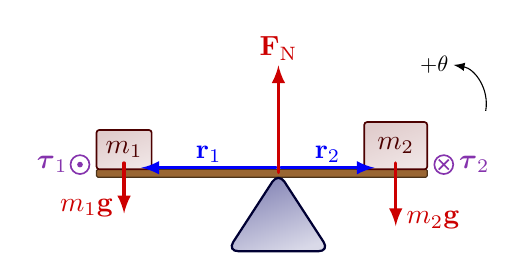
\begin{tikzpicture}
  \def\L{4.2} % length
  \def\w{1.3} % base width
  \def\h{1.0} % base height
  \def\F{0.8} % force magnitude
  \coordinate (O) at (0,0);
  \coordinate (M1) at (-0.55*\L,0.04*\h);
  \coordinate (M2) at ( 0.45*\L,0.04*\h);
  \coordinate (T1) at (-0.60*\L,0.1*\h);
  \coordinate (T2) at ( 0.50*\L,0.1*\h);
  \draw[thin,brown!40!black,fill=brown!80!black,rounded corners=0.5] (M1) --++ (\L,0) |-++ (-\L,-0.10*\h) -- cycle;
  \draw[mass] (M1) rectangle++ (0.7,0.5) node[midway] {$m_1$};
  \draw[mass] (M2) rectangle++ (-0.8,0.6) node[midway] {$m_2$};
  \draw[rvec] (O)++(-0.03,0.06) --++ (-0.55*\L+0.6,0) node[midway,above=-2] {$\vb{r}_1$};
  \draw[rvec] (O)++(0.03,0.06) --++ (0.45*\L-0.7,0) node[midway,above=-2] {$\vb{r}_2$};
  \draw[force] (M1)++(0.35,0.08*\h) --++ (0,-0.8*\F) node[above=2,left=0] {$m_1\vb{g}$};
  \draw[force] (M2)++(-0.4,0.08*\h) --++ (0,-\F) node[above=2,right=0] {$m_2\vb{g}$};
  \draw[force] (O) --++ (0,1.7*\F) node[above=-2] {$\vb{F}_\mathrm{N}$}; %$-(m_1+m_2)\vb{g}$
  \pic[scale=1] at (T1) {Tout};
  \node[mypurple,left=1] at (T1) {$\vb*{\tau}_1$};
  \pic[scale=1] at (T2) {Tin};
  \node[mypurple,right=2] at (T2) {$\vb*{\tau}_2$};
  \draw[thick,rounded corners=4,blue!20!black,
        top color=blue!40!black!50,bottom color=blue!40!black!15,shading angle=20]
    (-\w/2,-\h) -- (O) -- (\w/2,-\h) -- cycle;
  \draw[->] (M2)++(45:0.25*\L) arc(-10:80:0.12*\L) node[left=-1,scale=0.8] {$+\theta$};
\end{tikzpicture}


\end{document}